\documentclass{article}
\usepackage[utf8]{inputenc}
\usepackage{graphicx}
\graphicspath{{./YOLO11/}}

\begin{document}

\section{Introduction}

The core of this homework is object detection which draws bounding boxes of 
pigs in several images. My task is to implement a model that detects pigs 
in some angles of camera shots as accurately as possible.

\section{Training Procedure}

The dataset contains 7000+ training images and 2000+ test images. Each image
has a probability to be added with Gaussian noise, blur, and hsv variation, 
in order to make the model more robust.

\section{Model Description}

In this project, I use YOLOv11s as the base model, which is the latest version
of YOLO series that enhances the performance of object detection while maintaining
real-time inference speed.
I choose the YOLOv11 model due to its superior computational efficiency and 
detection accuracy. Its architecture consists of three main components:
\begin{itemize}
    \item \textbf{Backbone:} Utilizes an enhanced CSPDarknet structure for efficient multi-scale feature extraction.
    \item \textbf{Neck:} Employs a Path Aggregation Network (PAN) to improve information flow between different feature levels.
    \item \textbf{Head:} A decoupled head design that separately processes objectness, classification, and bounding box regression.
\end{itemize}
Moreover, so as to implement image augmentation, I change the image size to 1280.
Other hyperparameters are set by default.

\section{Experimental Results}

The following figures are the comparison of the results whether data is augmented.
It seems that the model doesn't perform better with data augmentation in this case.
I infer that the reason may be that all the training images are similar to test
images, so augmenting data only introduces noise that degrades the performance.
\begin{figure}[h]
	\centering
	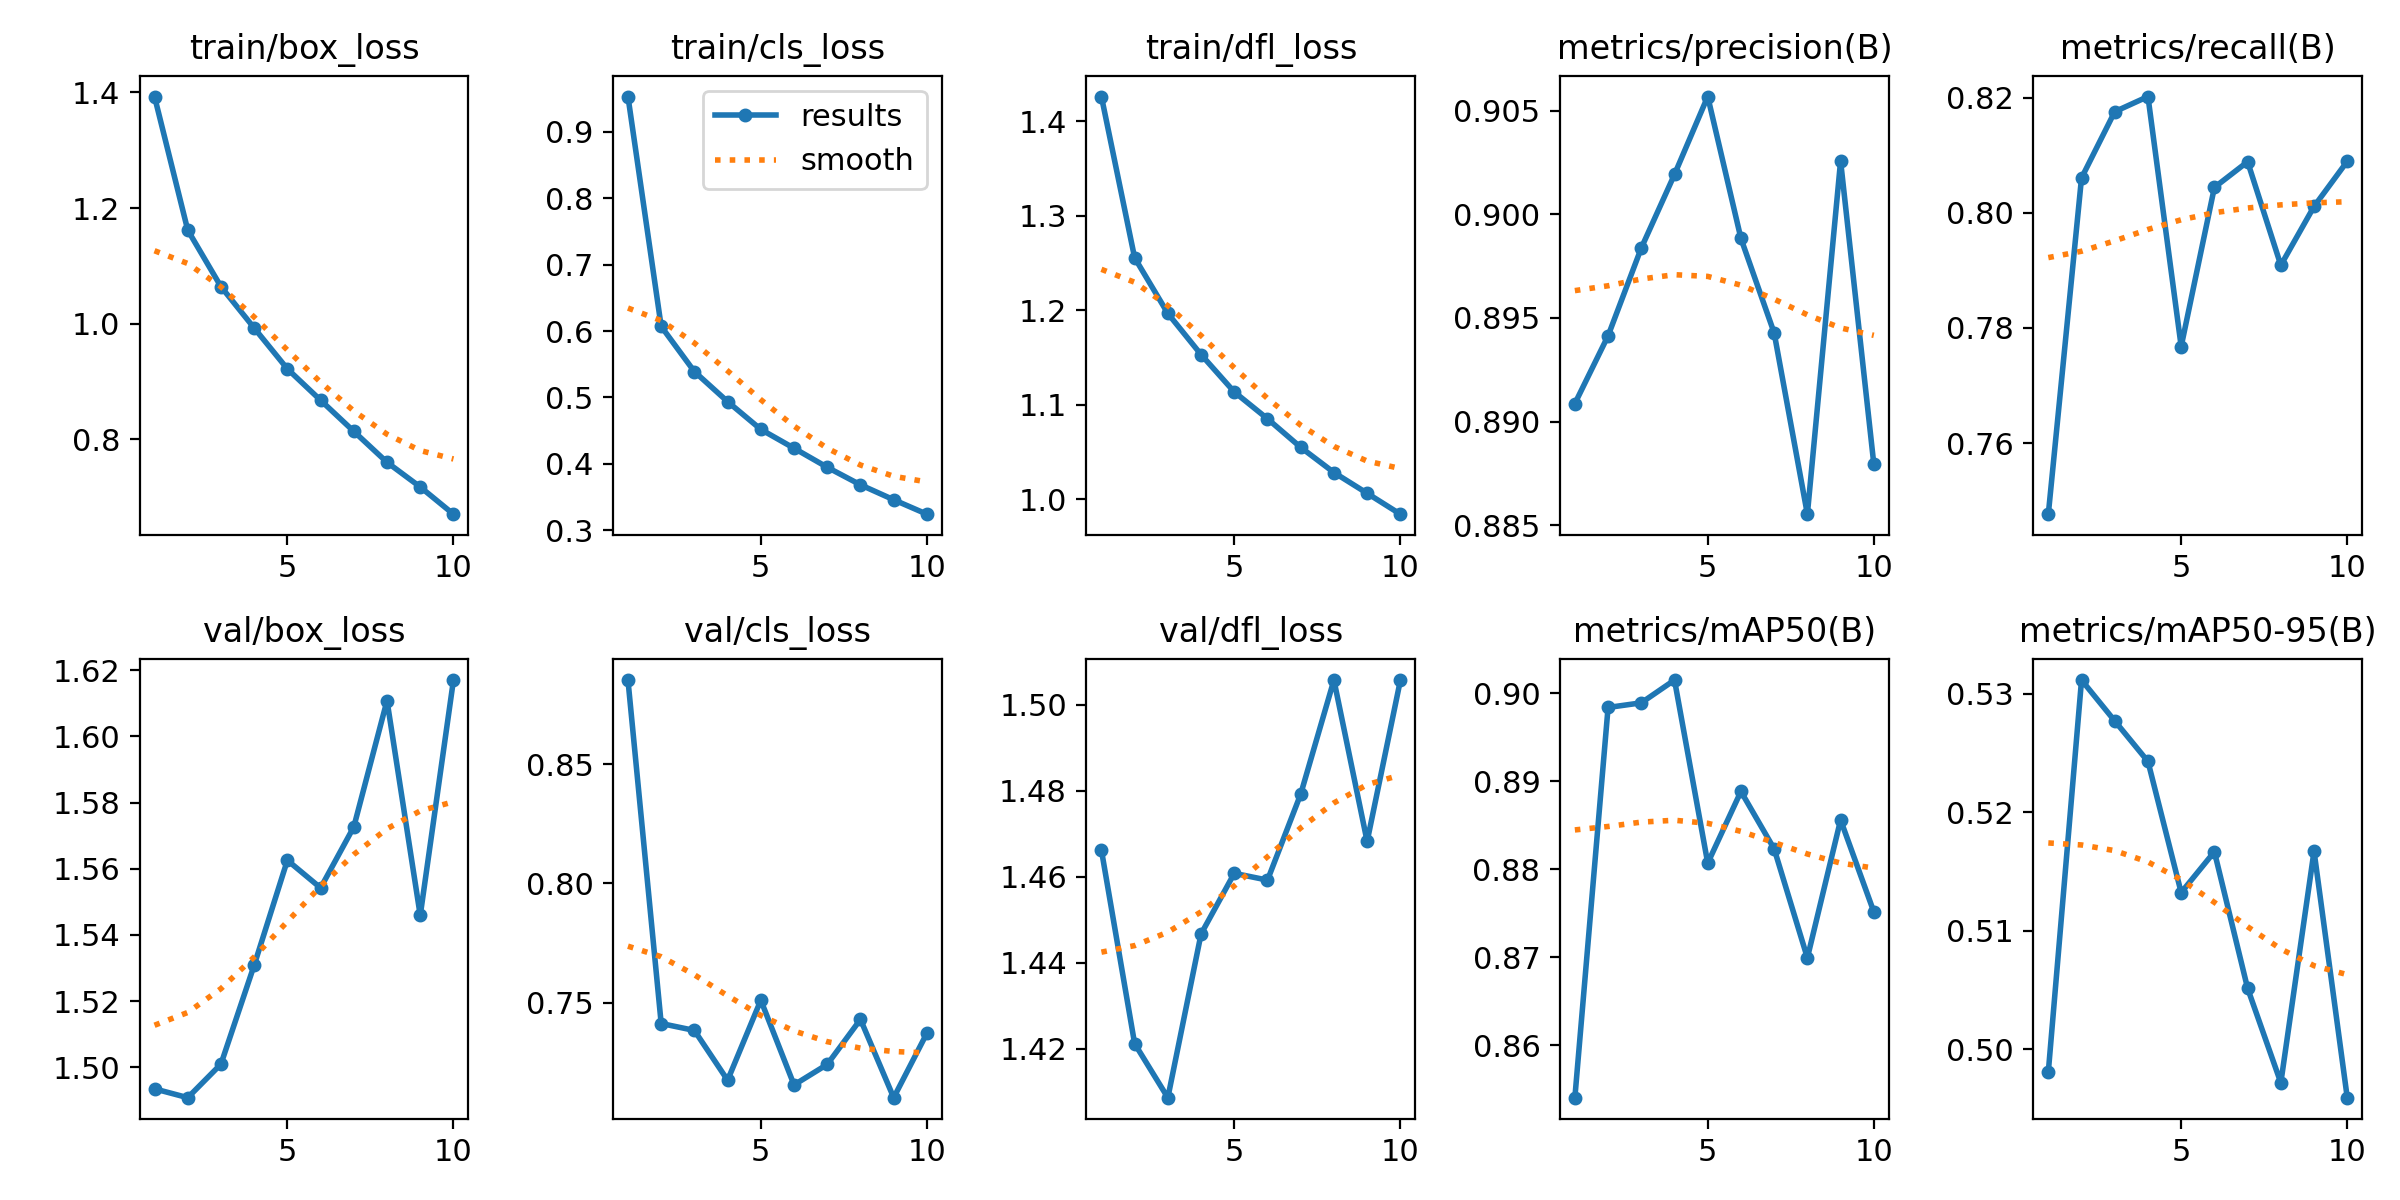
\includegraphics[width=0.8\textwidth]{ep10/results.png}
	\caption{Result of training 10 epochs}
	\label{fig:ep10}
\end{figure}
\begin{figure}[h]
	\centering
	
\includegraphics[width=0.8\textwidth]{ep10_no_aug/results.png}
	\caption{Result of training 10 epochs without data augmentation}
	\label{fig:ep10_no_aug}
\end{figure}

\clearpage
\section{Conclusion}

In this assignment, we successfully implemented a pig detection system 
using the YOLOv11s architecture. Through the experimental process, 
we explored the impact of data augmentation techniques, including 
Gaussian noise and HSV variations, on model performance.

Our results lead to a significant finding: for this specific dataset, 
data augmentation did not yield the expected performance boost. As 
analyzed in the results section, the high similarity between the training 
and testing distributions suggests that heavy augmentation may have acted 
as redundant noise rather than beneficial regularization. 

For future work, we plan to:
\begin{enumerate}
    \item Increase the number of training \textbf{epochs} to allow the model to fully converge.
    \item Experiment with \textbf{fine-tuning} specific augmentation parameters to find a better balance between robustness and accuracy.
    \item Evaluate the model's performance on a more diverse dataset to verify its \textbf{generalization} capabilities in real-world farming environments.
\end{enumerate}

\end{document}

